% vim: set foldmethod=marker :

% Cashner, villancico monograph, ch3
% on Gutiérrez de Padilla, Voces, las de la capilla
% 
% 2017-05-01      New version for book begun in Montrose
% 2017-08-04      Work resumed in Rochester
% 2017-12-14      Converted to Markdown
% 2018-01-22      Work resumed after ch2 revision
% 2018-02-08      Complete draft 
% 
% 2018-02-26      Begin revision 1
% 2018-04-04      Begin revision 2 after making floats
% 2018-04-10      Submitted to Grupo
% 2018-04-23      Revision 3 after Grupo comments
% 2018-05-09      Revision 3 completed, converted to LaTeX
% 2018-06-01      Complete draft sent to RLK, editor

% 2019-07-27      Trimming
% 2020-02-10      Final revisions

\part{Listening for Unhearable Music}
\label{part:unhearable-music}

\chapter{Christ as Singer and Song (Puebla, 1657)}
\label{ch:padilla-voces}

\epigraph
{Por el signo a la mi re, \\ 
puestos los ojos en mi, \\
a la voz del padre oí \\
cantar por puntos de llanto. \\
¡O qué canto!}
{Anonymous, \wtitle{Voces, las de la capilla} (Puebla, 1657)}

%{{{1 intro vignette
On Christmas Eve 1657 in colonial Puebla, the cathedral's tower bells had been
ringing for an hour when the first voices began to sing at 11 p.m.%
\begin{Footnote}
    The schedule was set by decree of the cathedral chapter,
    \sig{MEX-Pc}{AC 1633-12-30}:
    \quoted{Que a los maitines de nauidad deste año y de los venideros se
    llame desde las diez a las onze de la noche repicando la media ora y en
    lastra se toque la esquila para que puntualmente a las onze se enpiesen
    los dichos maitines \Dots}.
\end{Footnote}
Having heard the summons, the cathedral chapter gathered together with other
clerics, professors, landowners with their slaves, and common worshippers of
every caste, from Spaniards and their descendents down to indigenous people,
enslaved and free Africans, and people of mixed heritage.%
    \Autocites
    {AngelContreras:Puebla}
    {Lomeli:Puebla}
    {Sierra:UrbanSlavery}
Whether they came out of habit or obligation, or in sincere devotion, there was
little else for them to do but listen.
Fortunately the chapter had ensured that its chapelmaster, the priest Juan
Gutiérrez de Padilla, had prepared yet another sumptuous banquet of music,
including chant and Latin-texted polyphony both old and new.%
    \Autocites
    {Gembero:Padilla}
    {Hurtado:Padilla}
    {Stevenson:Padilla}
    {Miranda:PadillaLuz}
    {Gali:RitualesSonorosPuebla}
    {Swadley:VillancicoPhD}
The main attraction for many listeners, though, was the new set of Spanish
villancicos.

\index{Gutiérrez de Padilla, Juan|(}
\index{Puebla!Cathedral|(}
\index{villancico!liturgical function}
\index{Matins}
\index{villancico!audiences}
\index{social class}

As a cantor in Puebla Cathedral was intoning a Latin sermon of Pope Saint Leo
the Great---the first reading in the second Nocturne of Matins---the musical
chapel was preparing to raise their own voices.%
    \Autocites
    [175]{Catholic:Breviarium1631}
Holding handwritten notebooks with their individual performing parts for this
year's villancicos, they looked to Father Gutiérrez de Padilla for their cue.
When the chanting concluded with a descending cadence, the chapelmaster made
sure the chorus had the right starting pitches in their ears, perhaps with a
sung or played intonation.
He raised his hand and then lowered it to indicate the downbeat, and on one
side of the double-choir ensemble, the three voice parts (possibly three
individual singers) of Chorus I entered on the second beat, singing the word
\wtitle{Voces}.%
    \autocite[On indicating rhythm with the hand, see]
    [165--166]{Lorente:Porque}
The boy treble, adolescent alto, and tenor all sang this word high in their
registers, and the soft harmony of the opening G-minor (\emph{mollis}) chord
hung mysteriously the columns of the new cathedral's architectural choir.%
    \autocite{Merlo:PueblaCat}
Moving in the same rhythm, following the natural accents of the poetry, the
voices declaimed this text like a solemn choral recitative
(\musref{mus:Padilla-Voces-opening}):
\begin{quotepoem}
    Voces, las de la capilla,   & Voices of the chapel choir, \\
    cuenta con lo que se canta, & keep count with what is sung,  \\
    que es músico el Rey, y nota & for the King is a musician, and notes \\
    las más leves disonancias   & even the most venial dissonances, \\
    a lo de Jesús infante       & after the manner of Jesus the infant prince \\
    y a lo de David monarca.    & just as in the manner of David the monarch.
\end{quotepoem}
The other choir remained silent for these lines, as their notated parts
instructed them to heed the other chorus's admonition and \quoted{keep count} of
twenty-seven measures of rests until their entrance.

%{{{4 music Padilla voces opening
\begin{musicexample}
    \caption{Gutiérrez de Padilla, \wtitle{Voces, las de la capilla}, opening}
    \label{mus:Padilla-Voces-opening}
    \includefloat{Padilla-Voces-opening}
\end{musicexample}
%}}}4 

Some of those closest to the voices had already seen the poem in the published
commemorative pamphlet and may have spent some time puzzling over the complex
wordplay.%
\begin{Footnote}
    Though no imprint of villancico poetry corresponding to this Matins
    service has yet been found, several other imprints do survive from Puebla
    Cathedral for Christmas and the Conception of Mary during Gutiérrez de
    Padilla's tenure.
\end{Footnote}
A few of them recognized the poem from an earlier, but slightly different,
version they had seen in an imported print of villancicos from Seville.%
\begin{Footnote}
    \wtitle{Villancicos qve se cantaron en la S. Iglesia Metropolytana de
    Seville, en los Maytines de los Santos Reyes.  En este año de mil y
    seiscientos y quarenta y siete} (Seville, 1647), Puebla, private
    collection, courtesy of Gustavo Mauleón Rodríguez.
\end{Footnote}
These educated worshippers listened closely to hear how the chapelmaster, now
approaching his seventieth birthday and showing signs of age, would demonstrate
his mastery by realizing the poem's musical conceits in actual music.

The rest of the crowd heard and understood less, but recognized the opening
conceit of \foreign{voces}, and heard distinctly the phrase \foreign{que es
músico el Rey} and the references to David and \foreign{Jesús infante}.
As they looked past the choir to the newly decorated Altar of the Kings, filled
with images of Christ's birth and of celestial music, and as they heard the
solemn dialogue between choirs give way to a more lively texture, they worked
to imagine what sort of music the choir was singing about---the music of King
David with his lyre, the song of the Christmas angels, or the music they were
hearing this night in the heart of New Spain?

Thus began a tour-de-force of music about music, in which the composer and his
ensemble took a verbal discourse about music and turned it into a
\emph{musical} discourse about music.
When the first chorus refers to \quoted{what is sung}, they are referring to
more than the literal level of human music.
Instead, they point to \foreign{Jesús infante}---the child who is both the
\foreign{infante} or heir of the musician-king David and who is also God made
flesh as an infant, a child too young to be able to speak.

The next two chapters analyze and interpret families of villancicos that
represent Christ as both singer and song---this 1657 piece and another from
around 1660 by Joan Cererols of Montserrat.
Both invite hearers to listen for the harmonies between earthly, heavenly, and
divine forms of music.
Both families contain multiple settings of the same or similar texts: Gutiérrez
de Padilla's \wtitle{Voces, las de la capilla} is one of four known settings in
its family, while \wtitle{Suspended, cielos, vuestro dulce canto} by Cererols
is one of the best-attested families of villancicos with eight settings of
variant poetic texts through about 1700.%
    \Autocite
    [Both edited in][]
    {Cashner:WLSCM32}
These villancicos for Christmas connect Incarnation, voice, and creation, as
they invite hearers to consider human music-making as a reflection of
Christ's nature as the divine \quoted{Word made flesh} (\scripture{Jn 1}).
Both textual traditions build on an ancient theological trope of Christ as
\term{Verbum infans}---the infant, or unspeaking Word.
Christ the Word does not need to speak because God is already communicating
himself to humankind through the Christ-child's incarnate body.
The villancicos set by Gutiérrez de Padilla and Cererols turn this into musical
theology by imagining the baby Jesus not speaking, but singing; and by
considering Christ himself as the song being sung.

\index{villancico!families}
\index{theology!Christology}
\index{Incarnation}
\index{theology!of Word}
\index{\emph{Verbum infans}}
\index{villancico!dedications!Christmas}
\index{villancico!social function!contemplation}

In this chapter we will listen closely to the words and music of Gutiérrez de
Padilla's \wtitle{Voces, las de la capilla} to understand how the Puebla chapel
choir put their beliefs about music's power into practice through musical
performance, and to learn what this tells us about how Spanish Catholics
listened to music.
This villancico and other metamusical pieces related to it, I argue, trained
worshippers to listen past human music-making, to strain to discern the unhearable
higher music of the divine.
By representing the trope of Christ as singer and song through this genre of
sung poetry, the piece challenges listeners to hear the divine voice through the
voices of the chorus.
Within a Neoplatonic theological tradition, these pieces connected faith and
hearing by making Christ the Word audible through poetic and musical structures.
In a sense they \quoted{incarnated} the poetry and give it material form through
musical performance in a specific place and time.
At the same time they point beyond sounding music to higher forms of music.

\index{Neoplatonism}

This anonymous poem and Gutiérrez de Padilla's musical setting both demand and
reward detailed analysis.
In fact, that kind of close study is an extension of the same kind of listening
practice the piece was designed to inculcate.
The poem is cryptic even by seventeenth-century standards, but it was printed
and disseminated publicly, with the intent to communicate with some audience of
readers.%
    \Autocite[On the sociology and aural capacity of seventeenth-century
    Spanish audiences, with focus on sacred drama, see][]
    {DiezBorque:Publico}
Most likely, the poem was written specifically to be set by music, and was
designed to give a composer as many musical concepts to play with as possible.
Likewise, much of the composer's musical ingenuity would have only registered
with the most well-trained listeners, but the piece was performed as part of a
public liturgy that probably drew a large and varied congregation.

Gutiérrez de Padilla's metamusical villancico was a performance of musical
theology that challenged listeners to find the hidden connections between the
world of song and the world of spirit.
As the case studies in \partref{part:unhearable-music} will demonstrate, Spanish
chapelmasters also used metamusical villancicos socially to prove their craft
as master musicians.
In this way they established links of kinship to teachers and fellow musicians
who set the same or similar texts and developed the same kinds of
musical-theological tropes.
On the artistic level composers developed tropes for using music to represent
itself, vying with each other for the most overt, symbolically meaningful, and
moving displays of musical artifice.
As part of a theological tradition, the pieces on themes of heavenly music
manifest changing ways of thinking about the relationship between earthly and
heavenly music, in the midst of shifting understandings of the cosmos, the
human body, and society.
%}}}1

%{{{1 poem
\section{\quoted{Voices of the Chapel Choir} and the \quoted{Unspeaking Word}}

The anonymous poem evokes the musical voices of human singers, angelic choirs,
ancient prophets, and even the cries of the baby Jesus
(\poemref{poem:Voces-Padilla-1}, \ref{poem:Voces-Padilla-2}).% 
    \Autocite[37--38, 119--132]{Cashner:WLSCM32}
It demands a high level of intellectual engagement to tease out the intricate
conceit.
Exemplifying the technique of \term{conceptismo} after the manner of Góngora,
the poem's concept brings together the voices of the choir and the voice of
Christ.

\index{\emph{conceptismo}}
\index{Góngora, Luis de}

%{{{5 poem Voces 1,2
\begin{poemexample}
    \caption{\wtitle{Voces, las de la capilla}, from setting by Juan Gutiérrez
    de Padilla, Puebla, 1657 (\sig{MEX-Pc}{Leg. 3/3}), \emph{introducción}}
    \label{poem:Voces-Padilla-1}
    \includefloat{Voces-Padilla-1}
\end{poemexample}

\begin{poemexample}
    \caption{\wtitle{Voces, las de la capilla}, from setting by Gutiérrez de
    Padilla, estribillo and coplas}
    \label{poem:Voces-Padilla-2}
    \includefloat{Voces-Padilla-2}
\end{poemexample}
%}}}5

The second copla encapsulates the conceit: Christ is a musical
\quoted{composition} in which the divine chapelmaster \quoted{proves} his
mastery at creating \quoted{consonances of a Man and God}.
Like Spanish composers who established their superior musicianship over rivals
through the audition process known as \term{oposición}, God demonstrates his
mastery by creating concord between opposed elements.
Christ brings together infinite and finite (\quoted{maxima and breve}), and
creates a consonance to restore the discordant relationship between sinful Man
and the holy God by reconciling both in his own body.

\index{\emph{oposición}}
\index{harmony}
\index{consonance|see{harmony}}

The poem begins with the image of a \quoted{chapel}---that is, a musical
ensemble---performing before the king, like the Spanish \term{Capilla Real}.
This king \quoted{is a musician}, listening carefully for any defect in the
composition or performance: \quoted{he notes even the most venial dissonances}.
The poet connects the king with \quoted{David the monarch} and Jesus
as both an infant and the \term{infante} or heir (as a man, to David's throne;
and as divine, to the kingdom of God).
David was the paragon of Biblical musicians as both the traditional author of
the psalms and as founder of the first musical ensemble for worship in the
ancient Hebrew temple (\scripture{1Chr 25}).
The phrase \foreign{a lo de} (in the manner or style of) implies that the
child Jesus will be no less exacting a musical taskmaster than his ancestor.

\index{Madrid!Royal Chapel}
\index{David, King}

It only becomes clear later in the poem that the word \foreign{infante} also
points to another theological trope based on the double meaning of the Latin
word \foreign{infans} as both \quoted{infant} and \quoted{unable to speak}.
In this tradition, the Christ-child is \term{Verbum infans}---the
\quoted{unspeaking Word}, who does not need to speak because he himself
\emph{is} the Word.
This villancico's conceit treats both the Word and the child in musical terms,
so that Christ as the incarnate Word is a musical composition.
The child, then is depicted not as speaking but, through his cries, as
singing---making Christ both singer and song.

\index{Christ!as singer}
\index{Christ!as song}

To establish this metaphor, the poem uses a series of musical terms to present
Christ as the fulfillment of the Biblical prophecies made to and through David.
Christ's life \quoted{is putting notes to his lyrics} (\poemlines{8--9}), and
thus his life is recounted with the technical vocabulary for describing a
musical composition or performance.
Theologically, God had promised to David an heir to sit on his throne forever
and deliver his people (\scripture{2Sam 7}).
Through the prophet Isaiah he renewed this promise, declaring that a child
would be born \quoted{upon whose shoulder} would rest the \quoted{key} of
divine, eternal authority (\scripture{Is 22}).
As Biblical interpreters agreed, the complete fulfillment of these prophecies,
the culmination of all God's \quoted{centuries of heroic exploits}
(\poemline{8}) came not at Christ's birth, but at his death and resurrection,
traditionally thirty-three years later (plus three months and three days, to be
exact).%
    \Autocites
    [17]{Lapide:Gospels19C}
    [\sv{XXXIII}]{Ricciardo:CommentariaSymbolica}
    [\sv{XXXIII}]{Bongo:NumerorumMysteria}
    [for an earlier use of same number symbol by Gutiérrez de Padilla, see][]
    {Cashner:Cards}
The key of authority---\foreign{clave}---is the same word for clef; and it awaits
\quoted{the thirty-three}, suggesting some kind of musical measure.
In musical terms, the words of David and the prophets are just the lyrics;
Christ's life is the song.

\index{numerology}

The cryptic second section of the introduction (\poemlines{11--16}) depicts the
moment of Christ's birth as a musical performance.
Christ was born, the poem says, \quoted{years before the sign, \quoted{dexterity
in hope}}.
A \foreign{divisa} could be a sign of any kind but typically meant a heraldic
device, such as would appear on a crest or flag.%
    \Autocite[\sv{divisa}]{Covarrubias:Tesoro}
The motto \foreign{la destreza en la esperanza} sounds like a phrase from
Tacitus, \term{spes in virtute, salus ex victoria}.%
\begin{Footnote}
    Tacitus, \wtitle{Annals} II:20.
\end{Footnote}
Together with the other heroic vocabulary (\foreign{hazañas},
\foreign{destreza}, \foreign{divisa}), this phrase represents Christ as
fighting to save humanity, following after his ancestor David the giant-killer
(\scripture{1Sam 16}).%
\begin{Footnote}
    The preface to \autocite{Azevedo:Catecismo} uses the same kind of language
    to compare Charles I of Spain to King David in his battles to protect faith
    against heresy, calling the Creed \quoted{the signal and standard
    \addorig{señal y diuisa} that we who are of the Lord, and vassals of the
    faith, are to bear}.
\end{Footnote}
The sermons of Leo the Great read in Christmas Matins adjacent to this
villancico also characterize Christ's birth as the beginning of a battle with
the devil.%
    \Autocite[175]{Catholic:Breviarium1631}
The word \foreign{destreza} was used for musical heroes as well, to signify
virtuosity, especially compositional ingenuity.%
\begin{Footnote}
    \Autocites
    [\sv{destreza}]{Covarrubias:Tesoro}
    [in its musical sense, see the title of][]
    {Sanz:Guitarra}.
    Gutiérrez de Padilla used \foreign{destreza} and \foreign{hazañas} together
    to characterize the baby Jesus as a heroic rogue in his \term{jácaras} 
    of 1651 and 1659 (\sig{MEX-Pc}{Leg. 1/2}; \sig{US-BL}{PQ7296.A1V8}).
\end{Footnote}
It also recalls the technical term \foreign{diestro} in heraldry
(\term{dexter} in Latin and English, for the right-hand side of a crest, from
the perspective of the crest).%
    \Autocites
    [\sv{diestro}]{DRAE}
    [\sv{dexter}]{OED}
    {Johnston:Laterality}
The \foreign{divisa} could also be a musical sign such as a meter signature.
Theologically the \quoted{sign} may refer at one level to Christ's death on the
cross and on another level to Christ himself.

\index{heraldry}
\index{\emph{jácara}}
\index{Christ!as heir to King David}
\index{Christ!as chivalric hero}

In the estribillo (\poemlines{17--33}) the poem imagines the musical voices at
the moment of Christ's birth.
It brings together the whole creation in praise of Christ, panning down from
the celestial music of the spheres (\foreign{las distancias} or intervals, a
technical term in both astronomy and music), to the ensemble of \quoted{men and
beasts} (\poemline{20}) joining the angels.
The spheres sing \quoted{in one choir and the other} (\poemline{18}), like
Spain's polychoral ensembles.
The numbers here (\quoted{three by three, two by two, one by one}) at the most
literal level would seem to refer to the number of voices in a musical texture,
a cue Gutiérrez de Padilla does not miss.
As a theological symbol, \quoted{two by two} surely refers to Noah's Ark
(\scripture{Gn 5}), connecting it with both the animals in the Christmas stable
and to the biblical and patristic allegorical reading of the ark as the
church.%
\begin{Footnote}
    \scripture{1Pet 3:8-22}; \autocite[15]{Augustine:CivitateDei}. 
\end{Footnote}
\quoted{Three by three} probably refers to the traditional nine ranks of angelic
choirs.%
\begin{Footnote}
    See the entry for the number nine in \autocite{Bongo:NumerorumMysteria}; an
    example of the trope is the canon for nine choirs of angels on the
    frontispiece of \autocite{Kircher:Musurgia}.
\end{Footnote}
\quoted{One by one} could refer to humans or to Christ himself, particularly his
union of divine and human in a single body.
It is also possible that these lines form a chiasmus or ring structure, such
that \quoted{three by three} refers to the triune God, \quoted{two by two}
refers to animals, and \quoted{one by one} refers to humans, who must enter the
kingdom of God single-file.

\index{creation}

Thus far the poet has directed the listener's ear from attending to the chapel
choir singing in the present, to the ancient temple choir of David and the
voices of prophets through the centuries, up to the moment when the angels
led the song of \term{Gloria} at Christ's birth.
But all these voices, the poem now says, have been \quoted{awaiting the
opportune time, the one who was before all time} (\poemlines{24--25}).
The true music of Christmas is Christ himself, and thus the next lines represent
the voice of the baby Jesus.
The poem refers to the song that is Christ through solmization (\term{por sol},
\term{en mí}) and allusions to liturgical chants (\term{Gloria} and perhaps the
\term{Gratias agimus tibi}).
The musical imagery continues the conceit of the King as musician, a
\foreign{padre} (father, priest) like Gutiérrez de Padilla and most other
Spanish chapelmasters.
He sounds the pitch \term{A (la, mi, re)} in Guidonian solmization with his
voice as a tuning note or intonation (hence the description at the start of
this chapter).

\index{\emph{Gloria in excelsis}}
\index{musical topics!angels}
\index{solmization}

The listener now hears singing (\foreign{cantar}), in the form of a song
(\foreign{canto}).  
This is not the song of the creation chorus but the music they were
awaiting---the voice of Christ.
That voice sings in \foreign{puntos de llanto} (tones of weeping).
Musically this seems to play on \term{canto llano} (plainchant), while
theologically the reference to tears again highlights Christ's suffering.
Another translation of the contorted syntax here might suggest that the poetic
speaker actually \quoted{heard the voice of the Father singing}, that is,
\emph{through} the voice of the child.
This could also be a reference to the heavenly voice heard at Christ's baptism.%
\begin{Footnote} 
    \scripture{Mt 3:17; Mk 1:9-11; Lk 3:21-22}.
\end{Footnote}

After the invocation of \quoted{voices} at the opening, the reader or listener
has to wait all the way until this part of the poem to hear a direct reference
to hearing.
In the first fifteen lines of the estribillo there are only two simple verbs
that are not participles or part of a dependent clause: \foreign{aguardan} in
\poemline{23} and \foreign{oí} in \poemline{27}.
The first, \foreign{aguardan}, follows six verses describing the spheres, angels,
men, and beasts, who all \quoted{await} the time of Christ's birth.
After this, three more verses build up to \foreign{a la voz del padre oí} (at the
voice of the Father I heard).
This is the only use of the first person in the poem, and it makes the reader a
hearer.

At the center of this poem's concentric circles of voices is the Christ-child
himself.
The song the speaker hears is \quoted{as much to be seen (or admired) as to be
heard}---because the song and the singer are one and the same.
If the song is Christ, then, \quoted{the sign of \term{A (la, mi, re)}} is not
just a reference to musical tuning; it connects to the \foreign{divisa} of the
introduction to present Christ himself as a sign.

The estribillo concludes with the couplet, \quoted{Everything in Man is to
ascend/ and everything in God is to descend} (\poemlines{32--33}).
Because the estribillo is repeated after the coplas, this line also ends the
whole text in performance.
These verses use the musical structure of rising and falling musical lines (in
modern theoretical terms, a voice exchange) to epitomize the theology of
incarnation as an exchange between God and humanity.
This concept was repeated in every theological text on Christ's birth.
As Lapide puts it, Christ \quoted{lowered himself to the earth and flesh, in
order to lift us up to heaven. 
\quoted{Therefore}, says Saint Anselm, \quoted{God was made man, in order that
man might be made God}.}%
    \Autocite
    [670, on \scripture{Lk 2}; the quotation from Anselm is \quoted{Deus factus
    est homo, ut homo fieret Deus}.]
    {Lapide:Gospels19C}

\index{Incarnation}
\index{theology!Christology}
\index{counterpoint, symbolism}

To sum up this reading of the poem, then, the villancico began by drawing
listeners' attention to the voices of Christmas, and exhorting the singing
voices of the chapel choir to take note of their own singing while also
listening for \quoted{what is sung} on a higher level.
The piece connects Christ and David as musician-kings, with Christ as the song
that puts the prophetic \quoted{lyrics} of David and other Scriptural authors to
music.
After long waiting, at the \quoted{opportune time}, Christ was born into the
world to begin a battle \quoted{in hope}, a virtuoso performance fulfilled in
his death and resurrection at \quoted{the thirty-three}, upon the \quoted{sign}
of the cross.
Christ himself is the incarnate Word, and his infant cries are the true
\quoted{sign of A}, the \quoted{song} that sets the tone for all the other
voices, \quoted{in one choir and another} of the Christmas manger, and at the
Christmas liturgy in the time of the villancico's performance.
%}}}1

%{{{1 music
\section{Music about Music in the Voices of Puebla's Chapel Choir}

%{{{2 intro
The poem sets up a chain of echoes: what God spoke through the voices of David
and the other prophets reverberates in the song of the angels at the first
Christmas and especially the voice of the Christ-child. 
Ultimately all of this resounds through the actual \quoted{voices of the
chapel choir} singing in the present.
When Juan Gutiérrez de Padilla \quoted{puts notes to his lyrics}, he uses his
compositional ingenuity, and calls upon the virtuosity of his performers, to
turn a series of poetic conceits \emph{about} music into actual sounding music
that worshippers could hear.

On one level, the composer crafts musical structures that project the formal
structure of the poem at the levels of grammar, phrasing, and metrical
patterns.
He presents the words clearly according to their prosody and grammatical
structure, and sets them to memorable melodic and rhythmic patterns---well in
keeping with the directives of Trent.
The text-driven approach also shows the influence of Spanish popular and
theatrical traditions of singing poetry, especially practices of adapting stock
melodic formulas for \term{romance} poetry.

\index{music about music}

In addition to projecting the text in a way that makes it intelligible,
Gutiérrez de Padilla also uses two other text-setting techniques---text
depiction and text expression.%
\begin{Footnote}
    Peter Burkholder defines text depiction as \quoted{using musical gestures
    to reinforce visual images in the text}, and text expression, as
    \quoted{conveying through music the emotions or overall mood suggested by
    the text}: 
    \Autocite[207]{Burkholder:History}.
    I add to these terms the concept of text projection, and my conceptions of
    depiction and expression are somewhat broader, as depiction need not only
    be limited to \quoted{visual images} but includes numerological symbols,
    puns, and other such figures.
\end{Footnote}
The composer depicts the meaning of the words through musical symbols and
figures that correspond to concepts and imagery in the text.
These include the same kind of \quoted{madrigalisms} favored in
sixteenth-century Italy and Spain, as well as more arcane devices like
numerological symbols of an even older vintage.

\index{text depiction}
\index{text expression}
\index{madrigalisms}

In the technique of text expression, the composer goes beyond illustrating the
text and uses different stylistic registers and topics (that is, allusions to
other pre-existing types of music) to convey the meaning and feeling of the
text.
The composer dramatizes the text and uses music to heighten its rhetorical
power.
Text expression instills an affective experience in listeners that matches with
the goals of the poem.
Any vocal piece contains some element of text projection, depiction, and
expression; and these aspects often overlap.

In the case of this villancico, Gutiérrez de Padilla \emph{projects} the text at
the large scale through the formal structure of sections and harmonic motion;
and at the small scale through nuances of phrasing and rhythmic emphasis.
He \emph{depicts} the text by matching the musical conceits of the poem with
musical figures that correspond literally---essentially, puns.
The level of text painting seems to be the composer's main focus in this piece,
but he also \emph{expresses} the text through contrasting styles with different
affective associations, shaping the piece to build to a dramatic climax.
%}}}2

%{{{2 projection
\subsection{Projecting the Words}

Gutiérrez de Padilla projects the structure of the text through the distinct
sections of his setting.
The poem begins with an introductory section, which will be useful to label
\term{introducción} as many poetry imprints of other villancicos do.
This section consists of two six-line strophes, each followed by the same
\term{respuesta} or response of a four-line strophe.
The placement of rests and repeat markings in the performing parts makes clear
that the response is sung after each of the six-line strophes.
An \term{estribillo} follows, which is repeated after the two \term{coplas}.
Each of these sections is demarcated in the music with silence and a change of
texture, style, and rhythmic movement to match each part of the text.

\index{villancico!structure}
\index{\emph{introducción}|see{villancico!structure}}
\index{\emph{respuesta}|see{villancico!structure}}
\index{text projection|(}

The composer's treatment of the introducción's internal divisions, however,
breaks with the implicit structure of the poem as printed.
In the imprint from the earliest known version, a performance in Lisbon in
1642, the first sixteen lines are divided into four quatrains, with the same
text as Gutiérrez de Padilla's \poemlines{1--16} (see
\figref{fig:Lisbon-1642-Voces-imprint} below).
But in the version sung in Puebla in 1657, \poemlines{1--6} and
\poemlines{11--16} are grouped together and each is followed by
\poemlines{7--10}, now repeated as a \term{respuesta}.
Keeping the first six lines together emphasizes the central connection between
\foreign{la capilla}, \foreign{el rey}, \foreign{Jesús infante}, and
\foreign{David monarca}.
The phrasing and cadences in Gutiérrez de Padilla's setting make this grouping
seem natural, and this highlights the key difference between the villancico as a
literary genre meant to be read and the villancico as a musical genre meant to
be heard.

\index{villancico!musical genre!difference from poetic genre}

The piece's harmonic structure further helps articulate the form of the poem.
The piece is in mode I, in \term{cantus mollis}---that is, the one flat in the
key signature transposes the mode up a fourth; the final is on G and the Tenor
parts have a mostly authentic ambitus.
The internal cadences in the introduction are on G (\measure{19}), D
(\measure{27}), and G (\measure{44}); and the cadences at the end of the
estribillo and of both coplas are also on G.
These cadence points are in line with the prescriptions of contemporary
theorists for polyphony in this mode.%
    \Autocites
    [873--882, 883--885, 907--912]{Cerone:Melopeo}
    [364--406]{Judd:RenaissanceModalTheory}
    {Barnett:TonalOrganization17C}
Gutiérrez de Padilla uses harmonic conventions to punctuate the sections of the
poem and make its grammatical and rhetorical structure clear to listeners.

\index{mode}

The composer has paid close attention to both metrical patterns and details of
accentuation and diction, at the levels of strophes, verses, and individual
words.
For example, he sets the first two lines of poetry (\measures{1--10}) with
relatively long note values on the stressed syllables, creating a deliberate,
careful tone that embodies the poetic exhortation to \quoted{pay attention} to
what is sung.
For this poetry in \term{romance} meter, Gutiérrez de Padilla has the singers
declaim the eight-syllable lines in pairs, with emphasis on the assonant
even-numbered lines.
He has the singers pause briefly between verse pairs, and punctuates the
assonant lines with clear points of harmonic arrival.
He articulates the end of the strophes in the introduction with full cadences.
The musical setting thus aurally projects the text as though it were arranged
in lines of eight syllables with a \term{caesura}.
This structure mirrors the pattern of \term{romance} poetry as heard, rather
than as written in the narrow columns of villancico imprints.%
\begin{Footnote}
    \Autocites
    {Navarro:Metrica}
    [this structure is used in the \wtitle{Cantar de mío Cid}:][32--50]
    {MenendezPidal:Crestomatia}; 
    cf. also Old English and Germanic poetry.
\end{Footnote}

\index{\emph{romance} poetry}
\index{poetic meter}

The opening phrase demonstrates Gutiérrez de Padilla's subtle attention to the
sound and stress of the words (\musref{mus:Padilla-Voces-opening} above).
Chorus I sings the first word, \wtitle{Voces}, beginning on the second
subdivision of the ternary measure, with three minims for the first syllable and
two for the second.
That first word, in a common device of this composer's villancicos, is sung on
the second minim of the measure: thus the leader could conduct the downbeat,
cueing the singers to breathe, and then the chorus would sing their entrance. 
This first phrase, because of its high tessitura and irregular, offbeat rhythms,
seems suspended in the air in a way that would attract listeners' attention to
the ethereal \quoted{voices of the chapel choir}. 
The word \foreign{cuenta} (\measure{6}) is also sung on the second minim of the
measure and is then held for three minims, syncopated across the downbeat.
After this long note, like pulling back a spring, the metrical pattern is
released and the voices flow in even, regularly accented minims on \foreign{con
lo que se canta}.
For the next phrase (\foreign{que es músico el rey}) Gutiérrez de Padilla
creates the effect of an interjection, breaking the rhythmic pattern and
beginning this phrase, like the others, on the second minim of the measure.

\index{text projection|)}
%}}}2

%{{{2 depiction
\subsection{Depicting the Words}

The rest of the setting is as meticulously crafted as this opening phrase on the
level of text projection.
It is on the level of text depiction, though---representing the meaning of the
text through musical figures and symbols---that Gutiérrez de Padilla
demonstrates his full mastery of the craft.
For the word \foreign{cuenta} at the beginnging, he not only has one choir
literally count rests, but he also has the other choir sing this word on a
long, offbeat note that audibly captures the idea of \quoted{counting}.
It is notated as a blackened, dotted semibreve (that is, artificially perfected)
that leaps off the page as a visual indication to the singer to \quoted{keep
count}.
Gutiérrez de Padilla sets \quoted{the lightest dissonance} in \measures{14--19}
by creating just that: he has the Altus I suspend across the first minim of
\measure{18}, making a dissonant seventh against the Tenor's A that quickly
resolves to F sharp and then to a cadence on G in \measure{19}.

\index{text depiction|(}

In the \term{respuesta}, he continues this literal approach.
Where Chorus II sings about awaiting \quoted{the thirty-three}, Gutiérrez de
Padilla writes precisely thirty-three pitches for both of the sung vocal parts.
Just after the chorus sings that the whole world was \quoted{waiting} for
\quoted{the sign}, the composer uses the \meterC{} sign to indicate a shift to
duple meter (\measure{45}).
After this the musicians shift from free declamatory style to a more regular
rhythmic pattern, moving more quickly together in \term{corcheas} (modern
eighth notes).%
    \Autocite
    [This is the term used by Cerone and villancico poets (see \wtitle{Suban
    las voces al cielo} in \chapref{ch:zaragoza}):]
    {Cerone:Melopeo}
Here Gutiérrez de Padilla depicts what the words say by building up a point of
imitation \quoted{from one choir to the other} (\measures{45--50}) and then
creating polychoral dialogue (\measures{51--59}).
He sets the numbers in the poem literally, employing three performers for
\foreign{tres a tres}, two for \foreign{dos a dos}, and one for \foreign{uno a
uno}.

At the phrase \foreign{y aguardan tiempo oportuno} (\quoted{and they await the
opportune time}, \measure{60}), Gutiérrez de Padilla shifts meter signature
again, returning to ternary meter---in Spanish terminology, a new \term{tiempo}.
The theorist Lorente says this term can denote both the meter and the symbol
that sets the meter.%
    \Autocite[\range{bk}{2}, 149]{Lorente:Porque}
After the time signature \meterCZ, then, he begins a new lilting rhythmic
pattern that creates a sense of arrival in a new \quoted{time}.
He abruptly halts this movement at the end of the phrase, \foreign{quien antes
del tiempo fue} (\quoted{the one who was before time}, \measures{63--65}).
As Christ is \quoted{the first and the last} (\scripture{Rev 22:13}), this
halt is fitting.
Since Christ existed before all time theologically, Gutiérrez de Padilla puts
this phrase \quoted{before the time signature} musically.

\index{rhythm}

The musical conceits in the next lines of poetry shift the focus from rhythm to
melody, as the poem uses solmization symbols: \foreign{por el signo a la mi re,
puestos los ojos en mi}.
Likewise, Gutiérrez de Padilla's metamusical conceits play on the terms in the
most literal sense, realizing the solmization syllables in several ways at the
same time (\musref{mus:Padilla-Voces-alamire}).
Both Altus I and Tenor I sing the word \foreign{a} (\measure{67}) on the pitch
known by its Guidonian syllables as \foreign{A (la, mi, re)}.
On the words \foreign{la mi re} (\measures{68--69}), the Tiple I sings the
pitches D--C\sh{}--D, which could plausibly be sung to those syllables.
In the soft hexachord (which starts on F) the D would in fact be \term{la}.
The written sharp on C would alter it to a \term{mi} in \term{musica ficta}. 
The final D could be \term{re} in the natural hexachord (which starts on C);
thus, Gutiérrez de Padilla has spelled out \foreign{A la mi re}.
On the same words, the Tenor sings D--A--D: this would be \term{la--mi} in the
soft hexachord, then \term{re} in the natural hexachord.
At the end of this phrase (\measure{72}), all three voices sing the word
\term{mi} by literally \quoted{putting their eyes on \emph{mi}}: the Tiple and
Tenor sing \term{mi} on A (in the soft hexachord) and the Altus sings \term{mi}
on E (in the natural hexachord).

\index{solmization}

%{{{4 music Voces a la mi re
\begin{musicexample}
    \caption
    [Gutiérrez de Padilla, \wtitle{Voces, las de la capilla}, estribillo
    (\measures{66--72}): \quoted{The sign of \term{A (la, mi, re)}}]
    {Gutiérrez de Padilla, \wtitle{Voces, las de la capilla}, estribillo
    (\measures{66--72}): \quoted{The sign of \term{A (la, mi, re)}}
    (\term{mol}, \term{mollis}; \term{nat}, \term{naturalis})}

    \label{mus:Padilla-Voces-alamire}
    \includefloat{Padilla-Voces-alamire}
\end{musicexample}
%}}}4

The solmization villancicos discussed in \chapref{ch:intro} demonstrate that
Guidonian solmization was still a fundamental part of Spanish music instruction
through the eighteenth century. 
The syllables were used frequently enough that they later came to be used as
the Spanish names for pitch-classes in the seven-note scale (for example,
\term{sol} today is always the note G, which was historically \term{sol} in the
natural hexachord).
The prevalence of solmization is evidenced by books intended for specialists
(Cerone) and those for beginners, such as the 1677 guitar primer of
Lucas Ruiz de Ribayaz, as well as student notebooks in manuscript.%
\begin{Footnote}
    \Autocite{Ruiz:Luz}; examples of manuscript student notebooks are in
    \sig{E-Bbc}{M732/13--16}; see also \autocite{Cohen:NotesMiddleAges}.
\end{Footnote}
Even if fully trained singers did not often resort to the actual syllables in
reading music, they were trained in the system and could certainly have
recognized the Guidonian puns in this passage.

In the final couplet of the estribillo (\emph{Todo en el hombre es subir/ y todo
en Dios es bajar}, \measures{100--126}), Gutiérrez de Padilla matches the
theological concept of interchange between Man and God by creating an exchange
of musical gestures.
One gesture ascends in ternary rhythm and the other descends in duple
(sesquialtera) rhythm.
In the first of these gestures, for Man ascending, the voices ascend stepwise in
minims, in a lilting dotted rhythm with a strong ternary feel.
This is first heard in Altus I and Tenor I, \measures{98--100}, with the ascent
highlighted by having the Tenor move through F sharp.
In the second gesture, for God descending, all the voices move downwards in
emphatic duple rhythm with blackened semibreves.
The Tenor I has the highest number of blackened notes, singing a sequence of
descending intervals of decreasing size: first fourths (\measures{100--103}),
then thirds (\measures{108--112}), and finally seconds (\measures{118--122})
(\figref{fig:Padilla-Voces-TI-bajar}).
Just as the ascent pushed up into sharps, so the descent sinks down into added E
flats (Chorus I, \measures{100--104}).

%{{{4 figure coloration bajar
\begin{figure}
    \caption{Gutiérrez de Padilla, \wtitle{Voces, las de la capilla}, end of
    estribillo in Tenor I partbook: Coloration on figure for \quoted{God
    descending}}
    \label{fig:Padilla-Voces-TI-bajar}
    \includefloat{Padilla-Voces-TI-bajar}
\end{figure}
%}}}4

When Gutiérrez de Padilla juxtaposes these ideas in the full polychoral texture,
listeners can hear the fusion of both rising and falling melodic lines, and two
different rhythmic systems (\musref{mus:Padilla-Voces-subir_bajar}).
There is a clearly audible contrast between the rhythm of \quoted{God
descending} and that of \quoted{Man ascending}.
In the final cadence, the Altus I combines the two gestures at once by singing
the words \quoted{everything in God is to descend} to the music associated with
\quoted{Man ascending} (\measures{124--126}).
The passage musically embodies the central theology of the Incarnation: through
God's descent to become Man in Christ, Man may ascend to share in God's nature.

%{{{4 music estribillo subir/bajar
\begin{musicexample}
    \caption{Gutiérrez de Padilla, \wtitle{Voces, las de la capilla},
    estribillo (\measures{106--126}): Contrasting motives and rhythmic
    patterns for \quoted{Man ascending} and \quoted{God descending}}
    \label{mus:Padilla-Voces-subir_bajar}
    \includefloat{Padilla-Voces-subir_bajar}
\end{musicexample}
%}}}4

Gutiérrez de Padilla's literal approach to text depiction continues in the two
coplas.
Each of the two poetic coplas centers on a concept from music theory: the first
plays with the notion of a \foreign{peregrino tono} (\quoted{wandering song}, or
the plainchant \term{tonus peregrinus}); the second, on the contrasting
rhythmic values of \foreign{la máxima y breve}.
Gutiérrez de Padilla may also quote a fragment of the actual chant tone here,
as the stepwise descent A--G--F in the Altus matches the medial cadence of the
tone and the F--E--D in the Tenor and Tiple matches the final cadence
(\musref{mus:Padilla-Voces-peregrino_tono}, 
\figref{fig:Cerone-tonus_peregrinus}).%
\begin{Footnote}
    In other versions of the \term{tonus peregrinus}, the medial cadence matches
    exactly with the music of the Altus I (G--B\fl{}--A--G--F):
    \autocite[160]{Catholic:LiberUsualis1956}.
\end{Footnote}

\index{\emph{tonus peregrinus}}

%{{{4 figure tonus peregrinus
\begin{figure}
    \caption{The \term{tonus peregrinus} (\quoted{tono irregular o mixto},
    \quoted{octavo irregular}) in Cerone, \wtitle{El melopeo y maestro}, 354}
    \label{fig:Cerone-tonus_peregrinus}
    \includefloat{Cerone-tonus_peregrinus}
\end{figure}
%}}}4

%{{{4 music copla 1
\begin{musicexample}
    \caption{Gutiérrez de Padilla, \wtitle{Voces, las de la capilla}, copla 1
    (\measures{127--132}): Point of imitation quoting the chant \term{tonus
    peregrinus} on words \foreign{peregrino tono}}
    \label{mus:Padilla-Voces-peregrino_tono}
    \includefloat{Padilla-Voces-peregrino_tono}
\end{musicexample}
%}}}4

In the last phrase of this copla, when the poem speaks of Christ \quoted{going
up the octave} or theologically \quoted{ascending on the eighth day}, Gutiérrez
de Padilla creates an octave ascent across the voices, with the Tenor leaping
\pitch{D}{4}--\pitch{G}{4} and the Tiple continuing, \pitch{G}{4}--\pitch{D}{5}.
This octave also plays into the symbolism of the \term{tonus peregrinus},
which, as the eighth psalm tone, Cerone calls \foreign{octavo irregular}.%
    \Autocite[354]{Cerone:Melopeo}

The second copla emphasizes rhythm, using the note values of the \foreign{máxima}
and \foreign{breve}, to point to the union of eternal and temporal, infinite and
finite in Christ.
In medieval theory these were the longest and shortest note values, with the
maxima worth eight breves (the breve corresponding to a modern double-whole
note).
Gutiérrez de Padilla presents the basic concept of long versus short note
values through the lengthened note on \foreign{máxima} in the Tenor
(\measures{153--154}) over a long held note in the Bassus
(\measures{154--155}).
Ironically, each of these long notes is actually a breve
(\musref{mus:Padilla-Voces-maxima}).
How better, though, to express the unity between these opposites than by
vocalizing the name for one while singing the value of the other?
At a more arcane level, the whole first phrase of this copla
(\measures{147--156}) is ten measures (\term{compases}) long, which is
precisely equal to the length of a true maxima plus a breve.

%{{{4 music maxima
\begin{musicexample}
    \caption{Gutiérrez de Padilla, \wtitle{Voces, las de la capilla}, copla 2
    (\measures{152--156}): The word \emph{máxima} sung on a breve (original
    note values shown without bar lines)}
    \label{mus:Padilla-Voces-maxima}
    \includefloat{Padilla-Voces-maxima}
\end{musicexample}
%}}}4

\index{rhythm}
\index{music theory!symbolism}
\index{text depiction|)}
%}}}2

%{{{2 expression madrigal
\subsection{Expression and Madrigal Style}

This analysis shows that Gutiérrez de Padilla's setting as a whole is intimately
connected to the sound and meaning of the poetry.
The chapelmaster has his choir present the poem in a way that allows the words
to be heard clearly, reflecting their grammatical structure and the poem's
dramatic shape, while also embodying the conceits of the poetry in appropriate
musical symbols and even adding some musical puzzles of his own.
The contrasting styles in the piece would also work on a less intellectual, more
experiential level---that of text expression---to move the affections of
hearers.

\index{text expression|(}

The style of the estribillo, contrasting with the other sections, is like that
of a madrigal (\musref{mus:Padilla-Voces-madrigal}).
This section, then, is \quoted{music about music} not only in the way it uses
musical figures to represent music, but also by referring to multiple existing
genres and style of music within one villancico.
As the poem depicts the actual singing performed at the first Christmas,
Gutiérrez de Padilla uses the style of a genre used for convivial group singing.
The angels, planets, shepherds, and animals around the crèche are represented
not only as singing in the abstract---they are singing a madrigal.%
\begin{Footnote}
    The play on numbers, \quoted{three by three} and so on, is strongly
    reminiscent of the madrigal \wtitle{As Vesta Was from Latmos Hill
    Descending} by Thomas Weelkes (published in Thomas Morley's collection
    \wtitle{The Triumphes of Oriana} in 1601).
    The music of Weelkes and other English madrigalists did circulate in Iberia
    as far as Lisbon, to judge from the 1649 catalog of João IV.
\end{Footnote}

\index{Weelkes, Thomas}

%{{{4 music estribillo madrigal
\begin{musicexample}
    \caption{Gutiérrez de Padilla, \wtitle{Voces, las de la capilla},
    estribillo (\measures{48--59}): Evocation of madrigal style}
    \label{mus:Padilla-Voces-madrigal} 
    \includefloat{Padilla-Voces-madrigal} 
\end{musicexample}
%}}}4

By referencing different levels of musical style, Gutiérrez de Padilla maps
contrasting types of human music onto the contrast of earthly and heavenly
music.
The phrase \foreign{grave, suave y sonoro} seems to have been a stock description
of sacred music appropriate for liturgical worship.%
    \Autocite
    [On \foreign{suave} and other common vocabulary used for music in Spanish
    poetry, see][]{UribeBracho:OrfeoPhD}
The same words are used to describe the music of Christ as a musician in José
de Cáseda's \wtitle{Qué música divina} (see \chapref{ch:zaragoza}).
In 1682 a New Spanish nobleman used the same adjectives---\foreign{gravísima y
suavísima música}---to characterize the Matins music he endowed at Mexico City
Cathedral.%
    \Autocite[140--141]{Goldman:Responsory}
The music he requested, though, was specifically \emph{not} villancicos, but
rather only Latin-texted responsory settings.
This suggests that in this nobleman's mind the vernacular genre was not suitably
\quoted{solemn}.
In Gutiérrez de Padilla's piece, the term is used within a villancico to
refer to a higher form of music-making. 

\index{villancico!social status}

This stylistic reference also echoes the way the music of Christmas is portrayed
in contemporary Nativity images.
The composer's Andalusian compatriot Francisco de Zurbarán depicted two levels
of music in his \wtitle{Adoration of the Shepherds}, painted for the high altar
of the Carthusian monastery of Jerez de la Frontera in 1638--1639
(\figref{fig:Zurbaran-Jerez-Adoracion}).%
    \Autocite
    [Gutiérrez de Padilla had been chapelmaster of the cathedral of Jerez de la
    Frontera in 1612--1616:][]
    {Gembero:Padilla}
In heaven above, angels sing to the accompaniment of the harp, while below,
another angelic consort joins the company of worshippers in the stable, and they
sing to the accompaniment of the lute.
In Spain the harp was associated with both heavenly music and earthly church
music, and the lute, with musical genres performed outside of church, such as
the madrigal.
Villancicos crossed both domains, and therefore could incorporate references to
both styles within them.
This is analogous to the way Zurbarán's painting incorporates aspects of genre
painting---the representation of mundane details from everyday life---into a
representation of sacred history.%
    \Autocites
    [31]{Sanchez:Zurbaran}
    {Cherry:Bodegon}
    {Haraszti-Takacs:Genre}
Both visual and musical forms of crossover were especially fitting to represent
the Christmas moment when the \quoted{maxima} and \quoted{breve}, high and low,
were brought together, and the music of the heavenly chorus broke through to be
heard by humble shepherds.%
\begin{Footnote}
    Additionally, Zurbarán's image includes a bound lamb next to the manger as a
    symbol of Christ's fate as the paschal lamb, much as \quoted{the
    thirty-three} and other references in this villancico connect Christ's birth
    to his sacrificial death.
    The same trope may be seen in the Adoration of the Shepherds on the retable
    of Puebla Cathedral.
\end{Footnote}

\index{Zurbarán, Francisco}
\index{musical instruments!symbolism}
\index{visual art}
\index{text expression|)}

%{{{4 figure zurbaran pastores
\begin{figure}
    \caption
    [Francisco de Zurbarán, \wtitle{Adoración de los pastores}, retable of the
    Carthusian monastery of Jerez de la Frontera, 1638--39: The consort of
    heavenly and earthly music, harp above and lute below]
    {Francisco de Zurbarán, \wtitle{Adoración de los pastores}, retable of the
    Carthusian monastery of Jerez de la Frontera, 1638--39: The consort of
    heavenly and earthly music, harp above and lute below (Public-domain image
    of original in Musée de Grenoble)}

    \label{fig:Zurbaran-Jerez-Adoracion}
    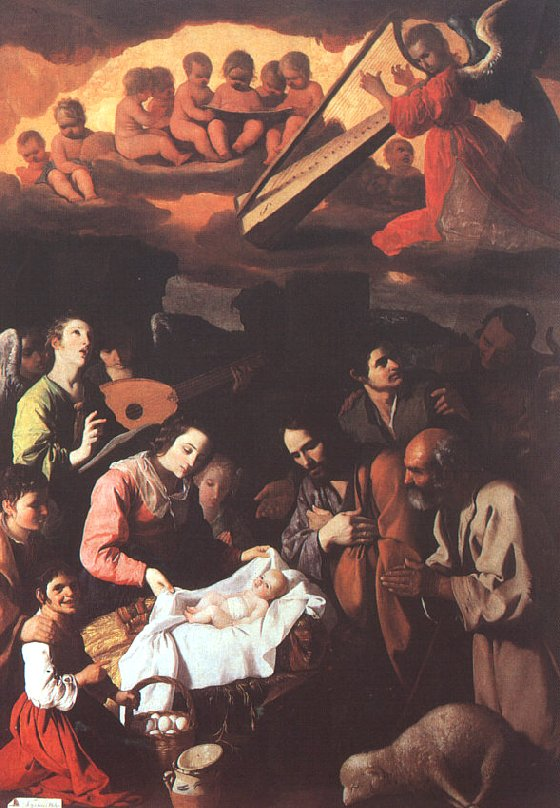
\includegraphics[width=\linewidth]{Zurbaran-Jerez-Adoracion}
\end{figure}
%}}}4
%}}}2
%}}}1

%{{{1 theology devotion Christ singer/song
\section{Devotion to Christ as Singer and Song}

By inviting hearers to listen for the voice of \foreign{Jesús infante},
Gutiérrez de Padilla's villancico presents a new, musical twist on an ancient
theological trope.
The concept of devotion to Christ as \quoted{unspeaking Word} reaches back to
the beginning of John's gospel, where Christ is \quoted{the Word made flesh},
through the subsequent elaborations of this concept of Augustine in the fifth
century and Bernard of Clairvaux in the twelfth.
A model sermon of Luis de Granada and the exegetical commentaries on the
Gospel infancy narratives by Cornelius à Lapide continue this tradition in
post-Trent Catholicism, in widely available texts that would have been familiar
to a university-educated priest like Gutiérrez de Padilla.
The historic libraries of Puebla's seminaries and convents included numerous
compendia of patristic commentaries on Scripture, model sermons, vernacular
devotional books, and learned Latin theological treatises
(\tabref{tab:puebla-compendia}).
\term{Ex libris} markings still identify the books from Puebla's 
Oratorian Society, to which Gutiérrez de Padilla belonged.%
    \Autocite{Mauleon:PadillaCivil}

\index{\emph{Verbum infans}}
\index{theology!of Word}
\index{Augustine, Saint}
\index{Bernard of Clairvaux, Saint}
\index{Lapide, Cornelius à}
\index{Granada, Luis de}
\index{theology!sources}
\index{theology!exegetical}
\index{theology!homiletical}
\index{Oratorians}

%{{{4 table compendia
\begin{table}
    \caption{Selected compendia of patristic exegesis and model sermons
    preserved from colonial libraries in Puebla's Biblioteca Palafoxiana and
    Biblioteca Lafragua}
    \label{tab:puebla-compendia}
    \includefloat{puebla-compendia}
\end{table}
%}}}4

The \term{Verbum infans} trope links the theology of \quoted{the Word} to
the theology of music.
It positions listening to music as a way of encountering Christ through the
sense of hearing, and its focus is on the voice of the infant Jesus himself.
Granada appeals to the sense of hearing throughout his Christmas sermon,
starting by asking the faithful to imagine the conversation of Mary and Joseph
on their way to Bethlehem.
After a detailed visual meditation on the scene in Bethlehem, he exhorts
worshippers to turn from sight toward hearing:
\begin{quoting}
    After the devout sight of the manger we open our ears to hear the music of
    the angels, of whom the Evangelist says, that when one of them had finished
    giving these very glad tidings to the shepherds, there were joined with him
    a crowd of the heavenly army, and that they all in one voice sang upon the
    airs praises to God, saying, Glory be to God in the heights, and on the
    earth peace to men of good will.%
        \Autocite[40]{LuisdeGranada:Xmas}
\end{quoting}
Even more important than these angelic voices, Granada preaches, is the voice
of the newborn Christ himself, \quoted{crying and trembling with cold in the
stable}.
Granada follows an ancient tradition of reading Wisdom 7---in which Christ's
ancestor King Solomon speaks about his own infancy---as a Messianic prophecy:
\quoted{I too am a mortal man like others, \Dots{} and the first sound
\add{\emph{voz}} that I made was crying like other children, because not one of
the kings had any different origin in their birth}.%
    \Autocites[37--38]{LuisdeGranada:Xmas}
    [Cf.][670, on \scripture{Lk 2}.]{Lapide:Gospels19C}

\index{Solomon, King}
\index{sight}
\index{voice!of Christ-child}

Granada explicitly compares the voice of this incarnate Word with music.  
The Dominican friar, an avid student of Catholic Humanism, presents Christ as
an orator and philosophical teacher, a \quoted{Master of
Heaven}---\foreign{Maestro del cielo}, the same term used for a musical
master:
\begin{quoting}
    Oh fortunate house!
    Oh stable, more precious than all the royal palaces, where God sat upon the
    chair \addorig{cátedra} of the philosophy of heaven, where the word of God,
    though made mute \addorig{la palabra de Dios enmudecida}, speaks so much
    more clearly, all the more silently it admonishes us!
    Look, then, brother, if you wish to be a true philosopher, do not remove
    yourself from this stable where the word of God cries while keeping silent
    \addorig{calladamente llora};
    but this cry is greater eloquence than that of Tully \add{Cicero}, and even
    than the music of the angels of heaven.%
        \Autocite[39]{LuisdeGranada:Xmas}
\end{quoting}
Granada's image of the infant Christ as an orator encapsulates the trope of
Christ as the \term{Verbum infans}.
For this passage he cites \quoted{a doctor}, and in fact the whole
passage is a paraphrase from Saint Bernard of Clairvaux.
When the friar calls Jesus \foreign{la palabra de Dios enmudecida} he is
glossing the term \term{Verbum infans} in Bernard's fifth Christmas sermon.
Bernard expresses the trope in this way:
\begin{quoting}
    But what kind of mediator is this, you ask, who is born in a stable, placed
    in a manger, wrapped in cloths like all others, cries like all others, in
    sum, who lies unspeaking as an infant \addorig{infans}, just as others
    are accustomed to do?
    A great mediator he is indeed, even in this seeking all the things that are
    for peace, not just going through the motions but working effectively.  He
    is an infant, but he is the infant Word \addorig{Verbum infans}, and not
    even in his infancy does he keep silent.%
        \Autocite[128A, Sermo V]{Bernard:Nativitate}
\end{quoting}
Bernard is himself drawing on an older tradition of the theology of the Word
going back to Saint Augustine, who in dozens of Christmas sermons reiterates
the trope of \term{Verbum infans doctor humilitatis}---the infant word, teacher
of humility.%
    \Autocite[1004, heading for sermon 187]{Augustine:SermonesPL}
The day of Christmas, Augustine preaches,
\begin{quoting}
    is called the Nativity of the Lord, when the Wisdom of God manifested
    itself unspeaking \add{or, as an infant}, and the Word of God without words
    sent forth a voice of flesh.
    That divinity which was thus hidden, was both signified to the Magi by the
    witness of Heaven, and announced to the shepherds by an angelic voice.
    This, therefore, is the day whose anniversary we celebrate in our ritual.%
        \Autocite[997, Sermo 185, In Natali Domini 2]{Augustine:SermonesPL}
\end{quoting}
As the master of a theology of communication through sign and signified (in
\wtitle{De doctrina christiana}), Augustine is teaching the faithful to ascend in
a Neoplatonic chain of signification.
The present-day Mass should point them to the signs through which Christ was
manifested at his birth, which in turn pointed to Christ himself as the
manifestation of God in \quoted{a voice of flesh}.

\index{theology!Christology}
\index{Incarnation}
\index{signification}
\index{Neoplatonism}
\index{Cicero}
\index{Humanism}
\index{communication}
\index{Christ!as newborn}

The \term{Verbum infans} trope fundamentally provides a way of thinking about
communication between God and humankind.
For Augustine, human communication was a reflection of the process of divine
communication. 
He used the voice to help his parishioners understand the Incarnation.
Prior to the Incarnation, he teaches, the Word of God existed from eternity,
like a human thought before it is expressed in words.
It \quoted{was not varied by punctuation marks whether short or long, nor drawn
together by the voice, nor ended by silence}.%
    \Autocite[1001, Sermo 187, In Natali Domini 4]{Augustine:SermonesPL}
But just as a thought is transferred into words without ceasing to be a thought,
so Christ took on human flesh while remaining divine.
The word makes communication possible because in speech, the abstract word is
expressed in a concrete, physical way:
\begin{quoting}
    A word \add{\term{verbum}; or, thought} that we carry in the heart, when
    joined with a voice \add{\term{vox}; or, speech, spoken word}, we bring
    forth to the ear, is not changed into the voice, but the whole word is
    assumed into the voice in which it proceeds, so that internally the idea the
    word makes intelligible remains, while externally the voice produces the
    sound that is heard.
    This word, then, brings forth in sound, what previously resounded in
    silence.  The word, upon being made a voice \add{or, upon being spoken}, is
    not changed into the voice itself, but rather, remaining in the mind's
    light, and having assumed the voice \add{speech} of flesh, it proceeds to
    the hearer, and does not leave the thinker.
    The word in silence is not thought by means of this voice \add{spoken word},
    whether it is Greek or Latin or whatever other tongue: but rather, the thing
    itself which is to be said, before all other differentiations of tongues, is
    understood in some naked manner in the chambers of the heart, from whence it
    proceeds, being spoken, to be clothed in the voice.%
    \Autocites
    [1002, Sermo 187, In Natali Domini 4]{Augustine:SermonesPL}
    [on Christ as \term{verbum}, see][872--889]{Lapide:Gospels19C}
\end{quoting}
In this conception the Christ-child embodies divine communication not through
spoken words, but through his very body.

\index{theology!of voice}

Augustine's theology of voice opened up rich possibilities for later interpreters
in the tradition to consider the Christ-child in specifically musical terms.
If Christ communicates God through his body, then one might imagine the
Christ-child as an oration given by a master speaker, as Lapide does in his
commentary on Luke:
\quoted{We hear God teaching and preaching from the chair \add{\emph{cathedra}}
of this manger, not by a word but by a deed: \Dots{} I have been made a little
one, of your bone and your flesh, I am made man, in order to make you God}.%
    \Autocite[673, on \scripture{Lk 2}]{Lapide:Gospels19C} 
If the voice is an apt metaphor for Christ as the divine Word, conveying the
divine nature to humanity, then Christ's actual voice would communicate doubly.
And if Christ can be both orator and oration, then surely he can be both singer
and song as well.

\index{rhetoric}

As the villancico \wtitle{Voces, las de la capilla} presents these tropes, the
Christ-child is the masterwork that proves the craft of the divine craftsman,
imagined as a chapelmaster in the Spanish fashion.
Bringing together \foreign{maxima} and \foreign{breve}, high and low
in the incarnate Christ, God the Father \quoted{proves} that he can form
\quoted{consonances between a man and God} (copla 2).
Thus on one level Christ is God's song, and \quoted{the Word} is envisioned not
as speech but as music.
Christ, then, takes the \quoted{lyrics} of his ancestor David, royal
chapelmaster, and \quoted{sets them to notes} (\poemline{7}) through his
heroic, sacrificial life.
He himself holds the \foreign{clave} (musical clef/key of authority); he
himself is the \foreign{divisa} (sign).

\index{Christ!as sign}
\index{Christ!as alphabet letter}

The note A is made a theological symbol of Christ himself as the sign, both
\foreign{signo} and \foreign{divisa}.
Both words draw on theological traditions that see Christ the Word as a
\quoted{sign}, and therefore even as a letter.
Covarrubias glosses the Spanish \foreign{divisa} with the Latin
\foreign{signum}, from the Greek \foreign{sēma}, sign. 
Likewise, Lapide calls Christ \quoted{the sign of reconciliation of the human
race to God}.%
    \Autocites
    [\sv{divisa}]{Covarrubias:Tesoro}
    [685--686, on \scripture{Lk 2}]{Lapide:Gospels19C}
Augustine connects the concept of the Word in John 1 to Christ's statement in
Revelation, \quoted{I am \emph{alpha} and \emph{omega}, first and last,
beginning and end} (\scripture{Rev 23}): \quoted{just as no letter comes
before \emph{alpha}}, he preaches, nothing precedes Christ or follows after
him, \quoted{for he is God}.%
\begin{Footnote}
    \shortcite
    [(MEX-Plf: 393-42010903) \range{vol}{10}, \folio{118\recto}, 
    In Natali Domini 2]
    {Augustine:Opera1555};
    \autocite[on \scripture{Rev 1}]{Lapide:Apocalypse1627}.
\end{Footnote}
In the villancico's terms, he is \quoted{the one who is before time}
(\poemline{24}).
The \foreign{divisa}, then, signifies the start of a new \foreign{tiempo}
(\poemlines{11, 23}).
The beginning of Christ's human life is the moment when idea is \quoted{clothed
in the voice} and communication becomes possible.

\index{Covarrubias, Sebastián de}
\index{signification}

If Christ himself is the sign, and if he is both singer and song, then the
\quoted{sign of A} is his singing voice---the cries of the infant considered as
music.
Spaniards believed that the first cry of newborn boys was the inarticulate
sound \emph{a} (pronounced like English \emph{ah}).
Covarrubias defines the letter A as \quoted{the first letter in order according
to all the nations that used characters, \Dots{} and this because of its being
so very simple in its pronunciation}.%
    \Autocites[\sv{A}]{Covarrubias:Tesoro}
This sound conveyed theological meaning about the nature of humankind:
\quoted{Thus it is the first thing that man pronounces in being born, except
that the male (since he has more strength) says A, and the female E
\add{pronounced \emph{eh}}, in which man seems to enter into the world,
lamenting his first parents Adam and Eve}.%
    \Autocites[\sv{A}]{Covarrubias:Tesoro}
By this account, keeping in mind Granada's description of Christ's newborn
cries, the baby Jesus first cried out with the inarticulate vowel \emph{A},
expressing in this sound his essence as \term{alpha} and \term{omega}, as
incarnate Word.
The sound of his voice in this context expressed Christ's identity as the son
of Adam, while also serving as a tuning note, or intonation, for a new song to
replace the \quoted{wandering song} given to \quoted{the first man}
(\poemlines{34--35}).
All the other voices of Christmas follow after and echo the voice of Christ.
Thus Christ in his cries performs the song that he himself is.
In the baby's cries could be heard \quoted{the voice of the Father} himself.
Parishioners hearing the Puebla chapel choir were challenged to listen for this
highest of all harmonies, the \quoted{consonances of man and God}.

\index{Christ!crying}
\index{Christ!as newborn}
\index{sin}
\index{\emph{alpha} and \emph{omega}}
\index{theology!of Word} 
\index{harmony}
%}}}1

%{{{1 pedigree
\section{Establishing a Pedigree in a Lineage of Metamusical Composition}

The high level of ingenuity, both theological and musical, in this villancico
makes \wtitle{Voces, las de la capilla} one of Juan Gutiérrez de Padilla's
master-works, in the early modern sense of a piece that proves the artisan's
mastery of his craft.
As such, the piece served a social function in addition to being an object of
devotion.
For the composer's fellow musicians, chapelmasters, and the educated elite of
Puebla, the piece demonstrated his skill and established his place in a
tradition of composition.
This setting is one link in a chain of homage and emulation, within a specific
family of villancicos.

Evidence survives for two previous villancicos beginning \wtitle{Voces, las de
la capilla} (\tabref{tab:Voces-Cantores-settings}).
The sources are a 1649 catalog entry for a setting by Francisco de Santiago
from the collection of Portuguese King John IV, and a 1642 poetry imprint of a
performance by the royal chapel in Lisbon
(\figref{fig:Lisbon-1642-Voces-imprint}).%
\begin{Footnote}
    \wtitle{Villancicos qve se cantarão na real capella do muyto alto, \et{}
    poderoso Rey Dom Ioamo IIII. nosso senhor. 
    Nas matina da noite do Natal da era de 1642} (Lisbon, 1642),
    \sig{P:Ln}{RES-189-3-P} (\itemnum{2}).
    Thanks to Álvaro Torrente for bringing this source to my attention.
\end{Footnote}
There is also a source for a variant version of the text, \wtitle{Cantores de la
capilla}, performed for Epiphany 1647 at Seville Cathedral and probably composed
by chapelmaster Luis Bernardo Jalón.%
\begin{Footnote}
    \wtitle{Villancicos qve se cantaron en la S. Iglesia Metropolytana de
    Seville, en los Maytines de los Santos Reyes.  En este año de mil y
    seiscientos y quarenta y siete} (Seville, 1647), Puebla, private
    collection, courtesy of Gustavo Mauleón Rodríguez.
\end{Footnote}
The 1642 Lisbon print represents the same branch of the textual family as
Gutiérrez de Padilla's 1657 setting, while the 1647 \wtitle{Cantores} text
forms a distinct branch.
In the 1649 catalog, among the \quoted{Christmas Villancicos of Fray Francisco
de Santiago} there appears the following entry:
\quoted{Vozes las de la capilla. solo. Ya trechos las distancias. a 9}.%
    \Autocite[caixão 26, \itemnum{674}]{JohnIV:Catalog}
The catalog only gives the text of the first line, but this matches the Lisbon
and Puebla versions (the corresponding music was lost with the Portuguese King
João IV's collection in the Lisbon earthquake and fires of 1755).

\index{João IV of Portugal}
\index{Jalón, Luis Bernardo}
\index{Royal Chapel, Portuguese}
\index{Lisbon, Royal Chapel}
\index{Seville!Cathedral}
\index{Epiphany}
\index{Santiago, Fray Francisco de}
\index{villancico!families|(}
\index{affiliation|(}

%{{{5 figure Lisbon imprint
\begin{figure}
    \caption{Earliest-known imprint of \wtitle{Voces, las de la capilla}
    family, Lisbon, 1642 (\sig{P:Ln}{RES-189-3-P}, \itemnum{2})}
    \label{fig:Lisbon-1642-Voces-imprint}
    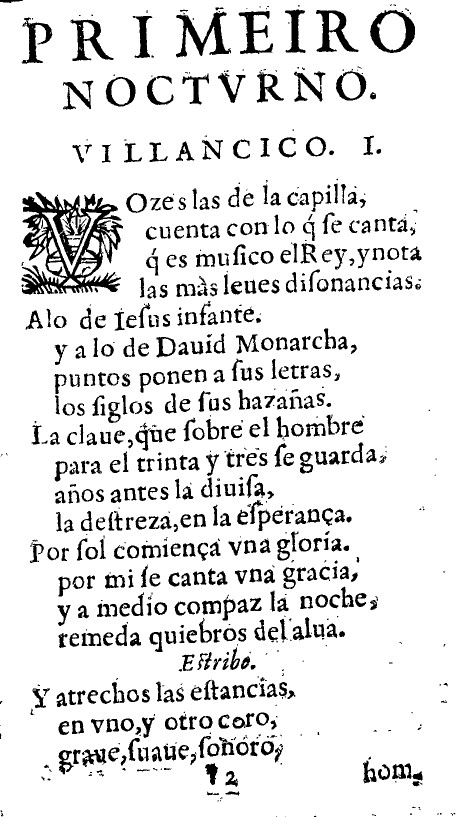
\includegraphics[height=0.5\textheight]{Lisbon-1642-Voces-imprint}
\end{figure}
%}}}5

%{{{5 table voces settings
\begin{table}
    \caption{Known settings of the \wtitle{Voces, las de la capilla}
    villancico family} 
    \label{tab:Voces-Cantores-settings}
    \includefloat{Voces-Cantores-settings}
\end{table}
%}}5}

Compared to the texts beginning with \term{Voces}, the 1647 text
\wtitle{Cantores de la capilla} is less complex, metrically regular, and
coherent 
(\tabref{tab:Voces-versions-1}--\ref{tab:Voces-versions-3}).
The 1647 \wtitle{Cantores} text only differs in small but revealing details
from both versions of \wtitle{Voces, las de la capilla}.
In the first four lines, Jalón's text has \foreign{Cantores} (singers) instead
of \foreign{Voces} (voices) and \foreign{Niño} (child) instead of \foreign{Rey}
(king).
Lines are added in the estribillo and a new copla is included that explicitly
reference the Three Kings, suitable for the performance of \wtitle{Cantores} at
Epiphany in Seville.
The end of the introduction in \wtitle{Voces} (\foreign{Por sol comienza una
Gloria}) is moved to serve as the final copla in \wtitle{Cantores}.
The whole \term{eco} section at the end of the 1642 \wtitle{Voces} is omitted,
so that the estribillo ends with the couplet \foreign{Todo en el hombre es
subir/ y todo en Dios es bajar}.

%{{{5 tables voces variants x3
\begin{table}
    \caption{Comparison of three extant variant texts of \emph{Voces, las de
    la capilla} villancico family (later correspondences to 1642 text
    underlined)}
    \label{tab:Voces-versions-1}
    \includefloat{Voces-versions-1}
\end{table}

\begin{table}
    \caption{Comparison of three extant variant texts of \emph{Voces, las de
    la capilla} villancico family, continued}
    \label{ref:Voces-versions-2}
    \includefloat{Voces-versions-2}
\end{table}

\begin{table}
    \caption{Comparison of three extant variant texts of \emph{Voces, las de
    la capilla} villancico family, conclusion}
    \label{tab:Voces-versions-3}
    \includefloat{Voces-versions-3}
\end{table}
%}}}5

\wtitle{Cantores} reads like an attempt to simplify and explain the dense
\term{conceptismo} of \wtitle{Voces}.
Where \wtitle{Voces} has an ambiguous or cryptic line, \wtitle{Cantores} has a
less multivalent one. 
The new poet has retained the technical terms and other key words used in the
first version of the poem, but has attempted to explain the metaphors, sometimes
in ways that change the meaning.
The connection of Christ's voice (\quoted{the sign of A}) and the \quoted{voices
of the chapel choir} is obscured, as the opening is changed to \quoted{singers
of the chapel choir}.
The key lines \foreign{a la voz del padre oí/ cantan por puntos de llanto},
are missing.
The theological connection between David and Christ as musician-kings is
weakened, and instead of saying that \quoted{the King is a musician},
\wtitle{Cantores} has \quoted{the child is a musician}---so that Christ is now
explicitly the creator of the music rather than himself being the Music
\emph{and} the musician.
Some of the musical terminology is deployed inaccurately:
It is hard to know what real meter might be indicated when \wtitle{Cantores}
has Christ the composer writing in \foreign{compás mayor} in a
\foreign{proporción abreviada} using a \foreign{clave con tres tiempos}.
When the compositor of \wtitle{Cantores} replaces \foreign{a la voz del padre
oí} with \foreign{con que mil maravillas vi}, he has replaced the central
reference to the act of hearing (\emph{oí})---the only first-person active verb
in the poem---with seeing (\emph{vi}), thus obscuring the poem's central
concept. 
Instead of listening to voices, the speaker of \wtitle{Cantores} is looking at
singers.

\index{\emph{conceptismo}}

Gutiérrez de Padilla's 1657 text, by contrast, is much closer to the 1642
\wtitle{Voces}, with only a few major differences.
First, as already noted, Gutiérrez de Padilla groups the verses in the
introduction as a six-line strophe followed by a four-line \term{respuesta},
which is then repeated after the rest of the introduction verses.
The 1642 text confirms the argument advanced above that the text of Gutiérrez de
Padilla's \term{respuesta} (the first time through) is meant to follow the sixth
verse, just as it is notated in the musical manuscripts.
But this grouping in six lines and adding a repeated section goes against the
patterns implied by the poem's metrical structure and appears to be a unique
interpretive decision, perhaps with the goal of creating dialogue between the
two choruses.
Second, Gutiérrez de Padilla, like Jalón, omits the \foreign{eco} portion of the
1642 text, ending with \foreign{Todo en Dios es bajar}.
Gutiérrez de Padilla does not use the same coplas as in the 1642 Lisbon or 1647
Seville prints (beginning \foreign{A suspensiones el cielo}), but rather includes
two completely different coplas (beginning \foreign{Daba un niño peregrino tono}).

The metrical patterning of the three texts suggests that Gutiérrez de Padilla's
version reflects an earlier stage of the tradition than either of the other
two, despite its later date.
First, Gutiérrez de Padilla's text alone features a \term{respuesta} section.
This structure was more commonly used in villancicos before 1640, though
Gutiérrez de Padilla, now in his senior years, continued to use the form in the
1650s.%
\begin{Footnote}
    Gutiérrez de Padilla, villancicos for Corpus Christi 1628, \wtitle{Salir
    primero de ti} (\sig{MEX-Pc}{Leg. 1/1}), and for Christmas 1653, \wtitle{A
    siolo Flasiquiyo} (\sig{MEX-Pc}{Leg. 2/1}).
\end{Footnote}
Second, the Puebla text alone includes a \term{linea de vuelta} (hinge line)
structure, a holdover from the form of the courtly villancicos of the sixteenth
century.%
    \Autocite{Navarro:Metrica}
In Gutiérrez de Padilla's text, the line \foreign{Y a trechos las distancias}
connects the end of the coplas (\foreign{de un hombre y Dios consonancias}) and
the start of the estribillo when that section is repeated.
The 1642 Lisbon \wtitle{Voces}, and the catalog entry for Santiago's
\wtitle{Voces}, both contain this same line (\foreign{Y a trechos las distancias}),
but the Lisbon version has different coplas from Gutiérrez de Padilla, and the
end of the coplas does not rhyme with \foreign{distancias}.
The rest of the estribillo has a consistent pattern in Gutiérrez de Padilla's
version: a series of fully rhyming, eight-syllable verse pairs, bracketed
before and after by half-lines, and followed by a \term{redondilla abrazada}.
The line \foreign{Y a trechos} breaks this pattern and only makes sense when
the estribillo is repeated. 

By contrast, the estribillo of \wtitle{Cantores} is much more irregular in
syllable counts and rhymes.
Its metrical irregularities are confined to the first portion of the
estribillo; after this the remainder is almost identical to \wtitle{Voces}.
Thus the first section appears \quoted{tacked on} to the more refined
pre-existing material in the second section.
Similarly, the 1642 Lisbon \wtitle{Voces} ends with an \foreign{eco} section in
a completely irregular meter, which develops unrelated themes and seems like a
superfluous addition.
These differences suggest that \wtitle{Cantores} was adapted from \wtitle{Voces}
with the goal of tempering its Góngora-like difficulty, and that it is not an
especially skillful adaptation.

If \wtitle{Cantores} is a later adaptation of \wtitle{Voces}, why did Gutiérrez
de Padilla revert to an earlier stage of the textual tradition?
The print of \wtitle{Cantores} was likely known to him, since the only
surviving copy survives in a binder's collection in Puebla. 
He must have had access to a source from the earlier textual tradition.
There is reason to believe that the three composers known to have set texts in
this family were personally connected in a professional network.
I propose that these chapelmasters deliberately chose to set their particular
versions in order to establish a kind of kinship with Santiago, the earlier
master (\tabref{tab:Voces-connections}).
Their musical relationships provided intergenerational connections for Spanish
musicians who were priests (like Gutiérrez de Padilla) or men of religious orders
(like Santiago), whose vow of celibacy precluded lineages of blood. 
These \term{maestros} learned and then transmitted their craft through
apprenticeship.
Chapelmasters were linked to their predecessors by a common practice of
assisting the incumbent in his final years, before succeeding to the position.
Parallel lines of succession with such interim assistantships in Puebla and
Sevilla are shown in \tabref{tab:Puebla-Seville-MCs}.

\index{kinship}

%{{{5 table voces connections
\begin{table}
    \caption{Connections between composers and settings of the \wtitle{Voces}
    villancico family}
    \label{tab:Voces-connections}
    \includefloat{Voces-connections}
\end{table}
%}}5}

%{{{5 table cathedral succession
\begin{table}
    \caption{Lines of succession at Seville and Puebla cathedrals, with
    interim succession plans in anticipation of incumbent's death}
    \label{tab:Puebla-Seville-MCs}
    \includefloat{Puebla-Seville-MCs}
\end{table}
%}}}5  

In Gutiérrez de Padilla's case, his apprenticeship began by serving as choirboy
and cantor at Málaga Cathedral and then assistant to the local chapelmaster
Francisco Vásquez (\circa{1602}--1608).
Unfortunately he was bested by the more experienced composer Estevão de Brito
in the competition to succeed his teacher.%
    \Autocites
    {Gembero:Padilla}
    {Stevenson:BritoE}
A new stage of apprenticeship began after Gutiérrez de Padilla emigrated to New
Spain, when he was selected in 1628 to assist the ailing Puebla chapelmaster
Gaspar Fernández.%
    \Autocite{Morales:Fernandez}
He composed the villancicos for Corpus Christi in that year, probably both as a
way to fill in for Fernández and to prove his own mastery.%
    \Autocite{Cashner:Cards}
He then succeeded Fernández after he died.
Now the master, Gutiérrez de Padilla cultivated his own apprentice in Puebla,
Juan García de Céspedes.
When Gutiérrez de Padilla's health began to fail in 1660, he signed a
\quoted{power of attorney} document giving legal rights to García, a member of
the Puebla ensemble whose name appears throughout Gutiérrez de Padilla's
partbooks.  
García then succeeded Gutiérrez de Padilla after his death in 1664.%
    \Autocite[237--238]{Mauleon:PadillaCivil}

\index{Málaga!Cathedral}
\index{Vásquez, Francisco}
\index{Brito, Estevão de}
\index{Puebla!Cathedral}
\index{Fernández, Gaspar}
\index{García de Céspedes, Juan}
\index{\emph{oposición}}
\index{rivalry}
\index{performers!boys}
\index{apprenticeship}

The Seville chapelmasters established a kinship-like lineage in the same way.
Francisco de Santiago first served as assistant in Alonso Lobo during his old
age in 1616.%
    \Autocites
    [\sv{Santiago, fray Francisco de}]{DMEH}
    {Stevenson:SantiagoF}
Santiago composed the \term{chanzonetas} (villancicos) for Christmas that year,
and then succeeded Lobo after his death in 1617.
When Santiago's time came and he was debilitated by a paralyzing medical
condition, the chapter called on Luis Bernardo Jalón to provide the music for
Christmas 1643, and Jalón inherited Santiago's position the following year.

\index{Seville!Cathedral}
\index{Santiago, Fray Francisco de}
\index{Lobo, Alonso}
\index{\emph{chanzoneta}|see{villancico}}

in these cases the lines of succession were established either by the composers
themselves or by the cathedral chapters, surely with the older master's
approval, since all these composers had at least a year to orient and train
their successors.
Musicians could also voluntarily demonstrate kinship.
Younger musicians could deliberately affiliate themselves with teachers and
paragons through composing musical homages (\tabref{tab:Padilla-homages}).
Francisco Vidales, organist in Gutiérrez de Padilla's Puebla chapel,
demonstrated his affiliation to the chapelmaster by writing a parody mass
based on one of his motets.%
\begin{Footnote}
    \Autocite{Koegel:Padilla}.    
    Cf. the successive reworkings of the same Victoria motet at
    Mexico City Cathedral through the eighteenth century:
    \autocite{Goldman:StileAntico}.
\end{Footnote}

\index{Vidales, Francisco}
\index{Victoria, Tomás Luis de}

%{{{5 table homages
\begin{table}
    \caption{Gutiérrez de Padilla's \wtitle{Voces} and younger composers'
    self-affiliation through homage to senior composers in their network}
    \label{tab:Padilla-homages}
    \includefloat{Padilla-homages}
\end{table}
%}}}5

It makes sense, then, that both Jalón and Gutiérrez de Padilla would try to
establish musical kinship with Santiago by adapting a text he had set.
Gutiérrez de Padilla likely knew Santiago personally from his own early career
in Andalusia, when he was climbing the ladder of prestigious positions in the
region, including Jerez de la Frontera (1612--1616) and the cathedral of Cádiz
(1616--1622).%
    \Autocite{Gembero:Padilla}
His years in Cádiz overlap with Santiago's tenure in Seville (1617--1643),
leaving about six years when the two chapelmasters in these two closely linked
port cities could easily have interacted personally or through correspondence.
The Seville composer's position at the helm of the flagship music program in
the Spanish world would have made him a prime target for emulation or
competition.%
\begin{Footnote}
    Gutiérrez de Padilla's \wtitle{Missa \quoted{Ego flos campi}}
    (\sig{MEX-Pc}{LiPol XV}) may even be an homage to Santiago's own lost
    mass of the same title, which according the João IV catalog, was based
    on the motet \wtitle{Ego flos campi a 8} by Nicolas Dupont, a Flemish
    composer in the Spanish Royal Chapel:
    \Autocites 
    [417, caixão 34, \itemnum{787}: \quoted{Missas \Dots{} Ego flos campi, a 8.
        \emph{Ferta sobre hum Motette de Niculas du Pont}};
    381, caixão 32, \itemnum{767}: \quoted{Ego flos campi, a 8, Niculas du
        Pont. \emph{De Nossa Senhora}}] 
    {JohnIV:Catalog}.
\end{Footnote}

\index{Jerez de la Frontera}
\index{Cádiz Cathedral}
\index{Dupont, Nicolas}
\index{Madrid!Royal Chapel}
\index{João IV of Portugal}
\index{villancico!families|)}
\index{affiliation|)}

%}}}1

%{{{1 conclusions: amazement
\section{\quoted{All Who Heard It Were Amazed}}

How can we understand the religious functions of this complex poetry and music
in light of both its social use to establish a pedigree and its context within
Catholic theological traditions?
What were listeners supposed to take away from the experience of hearing this
villancico?
Though the piece certainly could provide plenty of exercise for the intellect
of educated hearers and could serve to link its composer to a particular
heritage, I contend that the music's primary function for most of the Puebla
congregation was affective: it provoked awe and wonder in response to Christ's
Incarnation.

\index{affects}
\index{villancico!listener response}
\index{villancico!social function!worship}

This fit with the emphasis of a range of Catholic theological literature for
Christmas, from the catechism to sermons and commentaries.
The Catechism of Trent instructs pastors to teach the \quoted{admirable mystery}
of this article of faith by having \quoted{the faithful repeat by memory \Dots{}
that he \add{Christ} is God, who took on human flesh, and thereby was truly
\quoted{made man}---which cannot be grasped by our mind, nor explained through
words: that he should wish to become a human, to the end that we humans should
be reborn as children of God}.%
    \Autocite[50]{Catholic:Catechismus1614}
The incarnation of Christ, this passage suggests, was not so much a concept to
be understood as a miracle to be marvelled at.
The proper response to meditating on \quoted{all of these mysteries}, the
catechism says, would be \quoted{that with a humble and faithful spirit they
should believe, and adore}.%
    \Autocite[50]{Catholic:Catechismus1614}

\index{catechesis}

Written examples of teaching and preaching about Christ's birth demonstrate this
same devotional approach in their emphasis on wonder.
Even in the learned genre of a Latin Biblical commentary, Lapide stresses that
Christ's birth defies understanding: 
\quoted{The Word was made flesh, God was made man, the Son of God was made the
son of a Virgin.
This \Dots{} was of all God's works the greatest and best, such that it
stupefied and stupefies the angels and all the saints}.%
    \Autocite
    [50, on \scripture{Mt 6}]
    {Lapide:Gospels19C}
In a model sermon, Granada draws on all his rhetorical skills to exhort
worshippers to marvel at the sight and sound of Christ at his lowly birth:
\begin{quoting}
    Come and see the Son of God, not in the bosom of the Father \add{Jn 1}, but
    in the arms of the Mother; not above choirs of angels, but among filthy
    animals; not seated at the right hand of the Majesty on high \add{Heb 1},
    but reclining in a stable for beasts; not thundering and casting lightning
    in Heaven, but crying and trembling from cold in a stable.%
        \Autocite[37]{LuisdeGranada:Xmas}
\end{quoting}
Contemplating Christ's birth, Granada preaches, will cause anyone to be
\quoted{struck numb} with awe:
\begin{quoting}
    What theme, then, can cause any greater wonder? \Dots{} 
    \add{As Saint Cyprian says}, I do not wonder at the figure of the world, nor
    the firmness of the earth \Dots{}; I marvel to see how the word of God could
    take on flesh. \Dots{} 
    In this mystery the greatness of the shock steals away all my senses, and
    with the prophet \add{Hab. 3} it makes me cry out: Lord, I heard your words,
    and I feared: I considered your works, and I was struck numb.
    With good reason, indeed, you are amazed, Prophet: for what thing could
    surprise anyone more, than that to which the Evangelist here refers in a few
    words, saying, \quoted{She gave birth to her only-begotten son, and she
    wrapped him in some rags, and laid him in a manger, because she did not find
    another place in that stable}?%
        \Autocite[38]{LuisdeGranada:Xmas}
\end{quoting}

\index{senses!confusion}
\index{theology!devotional}

Spanish devotional music for Christmas seems designed primarily to cultivate
this same attitude of wonder.
Gutiérrez de Padilla's setting of \wtitle{Voces, las de la capilla} instills
wonder not only in the words but in the virtuoso composition and performance
of the music as well.
The villancico aims less to instruct than to amaze. 
This supports Mary Gaylord's argument that the goal of elaborate Spanish poetry
is \quoted{to produce effects of astonishment and awe conveyed by the Latin term
\emph{admiratio}}.%
    \Autocite[227]{Gaylord:Poetry}
Indeed, Gutiérrez de Padilla's piece specifically asks listeners to imagine a
song that is \quoted{as much to hear as to admire \add{\emph{admirar}},/ as much
to admire as to hear}.

The concept of \term{admiratio} is, in fact, central to the Christmas liturgy.
It is encapsulated in the fourth Responsory of Matins, \wtitle{O magnum
mysterium et admirabile sacramentum}:
\begin{quoting}
    \emph{Respond}. O great mystery and admirable sacrament, that the animals
    should see the newborn Lord, lying in the manger.
    Blessed Virgin, whose womb was worthy to bear the Lord Christ.\newline
    \emph{Versicle}. Greetings, Mary, full of grace: The Lord is with you.% 
        \Autocite 
        [175: \quoted{\emph{R}. O magnum mysterium, \et{} admirabile
        sacramentum, vt animalia viderent Dominum natum, iacentem in praesepio:
        Beata Virgo, cuius viscera meruerunt portare Dominum Christum.
        \emph{V}. Ave Maria, gratia plena: Dominus tecum}.]
        {Catholic:Breviarium1631}
\end{quoting}
In his sermon Granada alludes to this Responsory in terms quite similar to
those in Gutiérrez de Padilla's villancico, when he cries out, \quoted{O
venerable mystery, more to be felt than to be spoken of; not to be explained
with words but to be adored with wonder in silence}.%
    \Autocite
    [38: \quoted{¡O venerable misterio, mas para sentir que para decir; no para
    explicarse con palabras, sino para adorarse con admiracion en silencio!}]
    {LuisdeGranada:Xmas}

\index{Matins}
\index{Responsory}

This Responsory was probably paired with Gutiérrez de Padilla's \wtitle{Voces,
las de la capilla} in the Puebla Cathedral liturgy on Christmas Eve 1657.
Based on the position of this villancico in manuscripts, it was most likely
sung as the fourth villancico in the Matins cycle.
This means that in accord with a 1633 decree of the cathedral chapter the
villancico would have occupied the same liturgical time and space as the
Responsory \wtitle{O magnum mysterium}.
The chapter mandated that while \quoted{the lessons should be sung in their
entirety}, \quoted{the \emph{chanzoneta} \add{villancico} shall serve for the
Responsory, which shall be prayed speaking while the singing is going
on}.%
\begin{Footnote}
    \sig{MEX-Pc}{AC 1633-12-30}:
    \quoted{Que a los maitines de nauidad deste año y de los venideros \Dots{}
    se canten todas las liçiones yn totum sin dejar cossa alguna dellas y que la
    chansoneta sirba de Responsorio el qual se diga resado mientrass se
    estubiere cantando}.
\end{Footnote}
This villancico stood in between the lessons of the second Nocturne, which were
taken from a Christmas sermon of Leo the Great.
This means that after a cantor chanted the first lesson, a reader spoke the
mandatory liturgical text of the fourth Responsory above \emph{while} the chorus
sang this villancico.
The conjunction of texts may not have communicated much to the lay people
outside the walls of the architectural choir, but for the learned cathedral
canons, the simultaneous performance of the Latin prayer and Spanish song would
have deepened the hidden connections between the two.

\index{Responsory}
\index{villancico!performance practice}
\index{villancico!relationship to Responsory}

The Responsory evokes the scenario of the Nativity, with the animals gathered
around the manger, just as the villancico calls up the image of angels, beasts,
and humans joining together in song around the Christ-child.
In the quatrain that closes the estribillo, the lines \foreign{tan de oír y de
admirar/ tan de admirar y de oír} actually seem like a reply to the Responsory,
as though to say that the mystery of the Incarnate Christ certainly is an
\quoted{admirable} sacrament---that is, one that can be seen---but it is also
an audible sacrament.

\index{sight}
\index{hearing}

By calling devotional attention to the infant's voice in its musical version of
the \term{Verbum infans} trope, Gutiérrez de Padilla's villancico suggests that
listeners can encounter Christ through hearing.
The voices of the Puebla Cathedral ensemble's men and boys directed worshippers
to imagine the sounds of the angelic choirs and to contemplate a higher kind of
music in the incarnate Christ.
These higher forms of music would be audible only by faith, through the present
cathedral music which was its echo.

Worshippers in Puebla who listened while looking toward the altar, newly
decorated by Pedro García Ferrer, could combine the auditory gestures toward
heavenly music with a resplendent vision of Neoplatonic ascent.%
    \Autocites
    {Merlo:PueblaCat}
    {Gali:GarciaFerrer}
Starting on either side of the altar they would see paintings of shepherds and
Magi greeting the infant Christ.
Their eyes would be drawn upward to the central image of the Immaculate Mary
being assumed into heaven, greeted by a heavenly consort of angels playing
instruments and dancing in the round, in the light of the Holy Trinity
(\figref{fig:Puebla-Ferrer-BMV}).%
   \Autocite[The complex is in part a visual embodiment of musical encomium:][]
   {Schmidt:Lob_der_Musik}
The ascent to the heavenly realm, as depicted on the altar, began with an
encounter with Christ in the lowliness of his Incarnation. 
Gutiérrez de Padilla's bishop, Juan de  Palafox y Mendoza, encouraged this type
of devotion: his book \wtitle{El Pastor de Nochebuena} invites worshippers to
imagine themselves journeying with the shepherds to meet the newborn Christ.%
    \Autocite{Palafox:Nochebuena}

\index{visual art}
\index{art|see{visual art}}
\index{Puebla!Cathedral}
\index{García Ferrer, Pedro}
\index{sanctoral devotion!Mary}
\index{Palafox y Mendoza, Juan de}
\index{shepherds}

%{{{5 figure Puebla Cathedral
\begin{figure}
    \caption{Puebla Cathedral, retable by Pedro García Ferrer and studio,
    \wtitle{Assumption of the Virgin}, 1649, detail (Photograph by the
    author)} 
    \label{fig:Puebla-Ferrer-BMV}
    \includefloat{Puebla-Ferrer-BMV}
\end{figure}
%}}}5 

Journeying with the shepherds meant imitating their faith.
Lapide invites readers to learn from the shepherds' example: they did more than
just hear the good news announced by angels; they believed it and then
\quoted{went and told everyone what they had seen and heard}
(\scripture{Lk 2:20}).
For \quoted{however many might have approached the manger, and seen Christ, but
only those could have believed in Christ, whose hearts God had effectively
moved; while the others, taking offense at Christ's poverty, would have spurned
him}.%
    \Autocite[677, on \scripture{Lk 2}]{Lapide:Gospels19C}
Faith here means more than intellectual assent to a doctrine like the
Incarnation; it means being \quoted{moved} to receive Christ.

But imagining a journey to Bethlehem, as the Puebla retable and Palafox's
writings invited Puebla parishioners to do, was only a devotional aid in the
service of a real encounter with Christ at the altar.
Paraphrasing Saint John Chrysostom, Lapide writes, \quoted{That which the Magi
saw in the manger, in a little hut, with much veneration and fear approached and
adored, you perceive the same thing not in the manger, but on the altar}.%
    \Autocite[672, on \scripture{Lk 2}]{Lapide:Gospels19C}
Lapide cites Saint Cyril to say that \quoted{symbolically, the manger is the
altar, on which Christ in the Mass by consecration is as though born and
sacrificed}.
Despite these high theological ideals, though, in practice it was uncommon for
lay people to receive the Eucharist physically.
Instead, music could serve a mediating function connecting common people to the
church through the sense of hearing.
Devotional music could help worshippers experience intellectually and
affectively something of the wonder and mystery of the Incarnation at
Christmas.

\index{Eucharist}

This function fits with the instructions in the Roman Catechism that the mystery
of the Incarnation is more to be marvelled at than explained in words.
Granada makes the Christmas story into a call to heartfelt worship:
\begin{quoting}
    But consider, that if the angels on that day sang and solemnized this
    mystery with \emph{Glorias} and praises, giving thanks for the redemption
    that came to us from heaven, even though they themselves were not the ones
    redeemed, what should we do who are redeemed?
    If they thus give thanks for the grace and mercy given to strangers, what
    should those do who were redeemed and restored by it?%
    \Autocite[41]{LuisdeGranada:Xmas}
\end{quoting}
The devotee's response of awe, a central element of Christmas devotion,
surpassed private experience and motivated people to share their response with
others.
Music could both motivate this kind of experience and provide a way
to share it.

A villancico like \wtitle{Voces, las de la capilla} contributed to these
devotional goals by appealing both to intellect---the obscure conceits, the
musical puns---and to the affective faculty through its appeal to bodily,
communal reaction and participation.
Metamusical Christmas villancicos appealed to the hearing of worshippers on
several levels, and opened the possibility for them to listen in faith for the
voices of angels and the voice of Christ.
If the goal of Christmas music was to echo the historical voices of Christmas
and provoke the same kind of awestruck wonder, then we can understand the
efforts of poets and chapelmasters to impress and even confound hearers through
ingenious auditory artistry.
For the listeners in Puebla Cathedral on Christmas Eve 1657, their relationship
to the villancico \wtitle{Voces, las de la capilla} would mirror their
relationship to the mysterious and logic-defying theology of the Incarnation:
those who understood little could still be amazed greatly; those who strained
to understand more would only find themselves more in awe.

\index{Gutiérrez de Padilla, Juan|)}
\index{Puebla!Cathedral|)}
%}}}1

\endinput
